%!TEX root = ../main.tex

\chapter{Functional Connectivity Correlation between Infraslow and High Frequency iEEG Activities}
\label{chapter:ieeg-infraslow-hfo-correlation}

This chapter examines the concordance between infraslow ($<0.1$) and high frequency ($>50$ Hz) iEEG neural information flow throughout multiple phases of epilepsy using Granger causality and graph theory. Results on three epileptic patients show overlap in the epileptic network as observed in the high to infraslow, and from preictal to the interictal, to the visible ictus.

\section{Introduction}

Few studies have shown that infraslow EEG (IsEEG) could be used as an ancillary tool for the localization of the seizure focus in scalp 
\citep{leistner2007combined, miller2007ictal, murai2020scalp}.
Several groups have also studied the relationships among IsEEG, the classic EEG frequencies, and the gamma or higher frequency ranges 
\citep{modur2012seizure, wu2014role, thompson2016interictal, inoue2019interictal}. But the utility of very low-frequency recording in epilepsy has not been universally accepted \citep{gross1999intracranial}. Only a fraction of publications concerning IsEEG and epilepsy have employed any form of quantitative analysis \citep{modur2012seizure, thompson2016interictal, thompson2016ictal, murai2020scalp}, and none appear to have applied it to HFO and infraslow EEG on the same patient.

In several prior studies in our lab, Granger causality (GC) \citep{granger1969investigating} has been used as an analysis tool for intracranial EEG (iEEG) in the high frequency bands, and found widespread network activity prior to visible seizure onset \citep{adhikari2013localizing, epstein2014application}. 

In this study, we apply Granger causality (GC) and connectivity analysis to high frequency and infraslow activities throughout multiple phases of focal epilepsy, from preictal to interictal. Results show a striking consistency among the iEEG networks identified by GC at both high and IsEEG frequencies, along with the visual seizure onset; plus the persistence of this network during the pre-ictal, and interictal phases of epilepsy.  

\section{Materials and methods}
\label{sec:methods}

\subsection{Patients selection}
All the data were analyzed under protocols approved by the Institutional Review Board of the Emory University School of Medicine. Patients - A, B and C were chosen retrospectively based upon meeting the following criteria: an established history of medication-refractory epilepsy, absence of obvious anatomical lesion on 3 Tesla MRI, clinical confidence in the site of seizure onset by contemporary intracranial EEG (iEEG) features and ancillary studies, and long-term improvement in clinical seizures following a focal invasive procedure. Additional data included positron emission tomography (PET), neuropsychological assessment, and if indicated, single photon emission computed tomography (SPECT), magnetoencephalography (MEG) or functional MRI (fMRI) mapping. All three patients had striking improvement (1) or prolonged remission (2) following invasive procedures.

Patient A had no known clinical seizures following bilateral mesial temporal electrode explantation, or for 18 months afterwards. Over the subsequent 6 years, seizures have been substantially milder and rarer than before the implantation. Prior to selection for the current investigation, this case had been assessed as a rare instance of long term remission related to implantation of intracranial electrodes \citep{katariwala2001remission, schulze2010seizure} . The striking and prolonged clinical improvement was considered strong confirmatory evidence for seizure origin at the site of implantation.% Patient B is GA

Patient B elected responsive neural stimulation following recording of electrographic seizure onset at a site where tissue ablation was considered to have high risk of permanent neurological deficit; this has resulted in sustained reduction in symptomatic seizures for  years.
% Patient C is QM

Patient C  has been in complete remission (Engel 1A)
for 4 years following laser ablation along the track of the electrode that recorded electrographic seizure onset 
% Patient A is WD


\subsection{IEEG recording}
Patients underwent implantation of depth electrodes, subdural grids, and/or strip electrodes (Ad-Tech Medical, Racine, USA) in various combinations according to the individual pre-surgical localization hypothesis.  Recordings were made with an XLTEK system (Natus Medical, San Carlos, CA, USA) using up to 128 electrodes. 

\begin{figure*}
\centerline{
	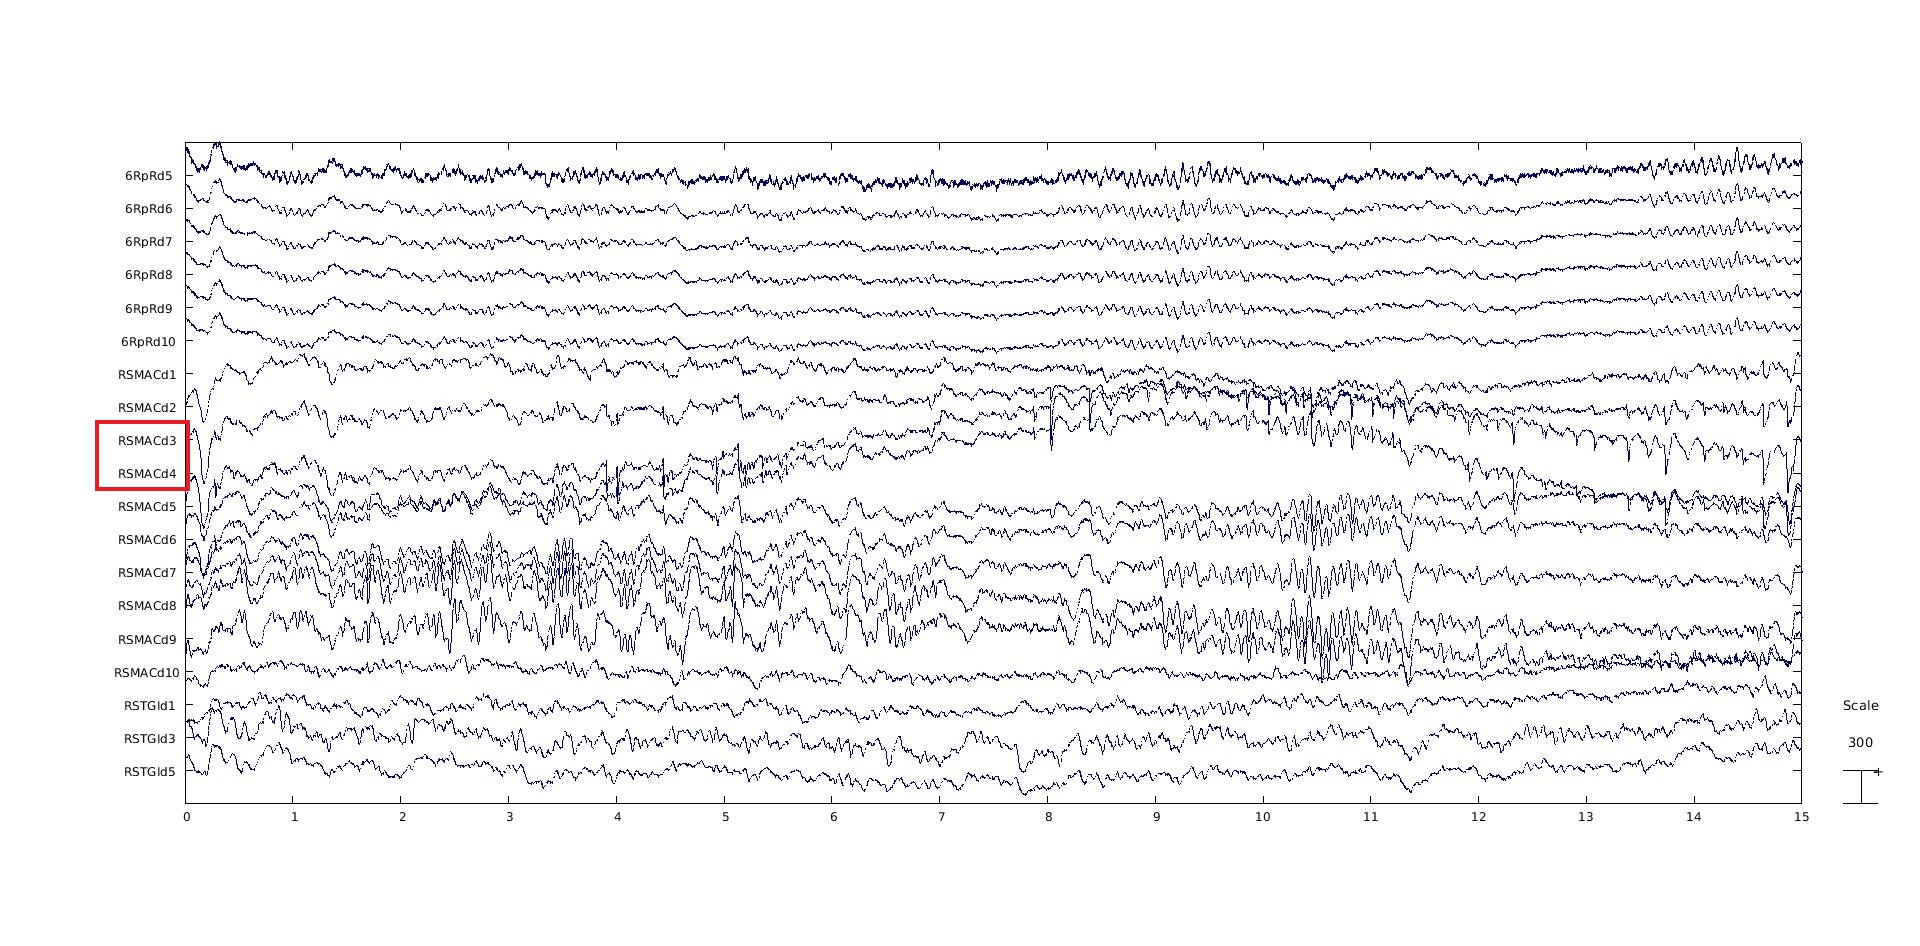
\includegraphics[height = 3.5in]{Plots/Patient_C_iEEG_rawdata_sample.jpg}
	}
	\caption{The unfiltered iEEG time-series shows spikes riding on top of slower waves on seizure onset electrodes in pre-ictal and ictal period. The red box highlights the seizure onset (SO) electrode.}
	\label{fig:rawdata_patient_c}
\end{figure*}

Initial oversampling and hardware antialiasing filters were followed by linear phase FIR filters with an order of 30, set to just below the Nyquist frequency for the final sampling rate of 500 or 1000 Hz. The Natus digital preamplifiers were specified to a lower frequency limit of 0.01 Hz, but no filtering was applied during download of wideband European Data Format (EDF) data for analysis. Visual identification of the iEEG seizure focus was performed according to current criteria \citep{andrzejak2015localization,grinenko2018fingerprint,gnatkovsky2019two} and the results of invasive therapies or procedures. Figure \ref{fig:rawdata_patient_c} shows the IEEG time-series on a few electrodes including the SO electrodes on a representative patient. The spikes are on top of slow waves. Similar infra-slow wave patterns relevant to seizure onset electrodes have been reported in \citep{rampp2012ictal}.



\subsection{Data pre-processing}
The iEEG time-series data were filtered using forward and backward finite impulse filters (FIR) in EEGLAB \citep{delorme2004eeglab} for its simple design, intrinsic stability and free of phase distortion. The data were band-pass filtered at a cutoff of 50 Hz to Nyquist frequency (half of the sampling frequency) for high frequency oscillations (HFOs) analysis and cutoff for infra-slow oscillations (ISO) were 0.01 Hz and 0.1 Hz. Temporal mean was removed from the time-series before advanced mathematical calculations. Pre-ictal data samples for high frequency activity were taken for 64, 69, and 54 seconds ending 1-2 seconds before visible seizure onset for patients A, B and C. Variable length of data segments were considered for different patients due to the artifacts present in the data. Similarly, 1550, 113 and 330 seconds data samples were analyzed for inter-ictal iEEG recording. For low frequency activity, data samples were selected visually to correspond to the beginning and the end of a baseline shift that coincided or overlapped with the visible seizure onset and was congruent with it in multiple electrodes.

\subsection{Time frequency analysis}
The wavelet based spectral power was computed from unfiltered iEEG time-series to investigate when and how the power changes for high frequency oscillations and infra slow oscillations in the seizure onset electrodes. We did not study the wavelet power for all the electrodes, for pre-ictal and interictal periods separately, as previously done in \citep{adhikari2013localizing} for high frequency oscillations. The aim of time frequency analysis is to confirm the significant high and infraslow oscillations in these iEEG time-series. This facilitates meaningful quantitative spectral interdependency analysis.

\subsection{Granger causality}
We computed pairwise Granger causality spectra and graph measures, as directed functional connectivity matrices to examine the strengths and directions of causal interactions in the frequency domain, among multi-channel digitized iEEG time-series \citep{dhamala2008analyzing}. Granger causality as computed in the time domain is the statistical technique that relies on the concept of temporal precedence of cause before effect and is based on the prediction of future behaviors using the past records \citep{granger1969investigating}. If the past of one time series X1 can help predict another time series X2 better than using the past of X2 alone, then X1 is known to have a causal influence on X2. Due to the difficulty of finding an optimal model order in the parametric pairwise approach, we used both non-parametric and parametric approaches at different model orders and selected the model order that yielded the lowest power difference. Accordingly, we obtained the optimum model order 8 for our analyses. Time domain Granger causality was obtained by integrating in the infra-slow frequency range and high frequency range as specified above.
%We would consider this method helpful in SOZ prediction if the leading visual electrodes and the strongest high-frequency and low frequency electrodes are identical.

\subsection{Graph measures}
Graph measures were computed from the time domain Granger causality matrix as the adjacency matrix using the BCT toolbox \citep{rubinov2010complex} with a threshold of 40\% above the maximum Granger causal flow. The electrodes were considered as the nodes and the causal relations between nodes were considered as the edges. Three centrality measures, betweenness, degree and closeness were computed to study the importance of SO electrodes in the network. Betweenness measure was computed for all the high-frequency and infraslow GC spectra from preictal to ictal period to study the number of paths SO electrode lies in the network graph. This represents the SO electrode's ability to make connections to other groups of brain areas \citep{chiang2014graph,wang2008betweenness}
Likewise, ‘Degree’ measures the number of edges of a node, and nodes with higher edges act like a hub of activity. Closeness centrality is the inverse of the sum of all shortest paths to other nodes. A higher closeness value corresponds to faster information spread throughout the network. For directed graphs, the closeness value is called ‘Incloseness’. Clustering coefficient is the measure of segregation of the network.


\section{Results}
\label{sec:results}

\subsection{Time frequency analysis}
We focused our study on high frequency oscillations and infra-slow oscillations in preictal and interictal periods. Figure \ref{fig:high_pass_filtered_preictal_patient_c} provides a sample iEEG time series after finite impulse filtering (FIR) for high frequency oscillations. This data includes clinically identified seizure events illustrating HFOs as one of the biomarkers of seizure onset electrodes. Even though HFOs were observed in all channels in both preictal and interictal states, the evolution of HFOs was distinctly visible in the SO electrode and later extended to multiple channels, mostly in preictal period.

Figure \ref{fig:infraslow_wave_patient_c} represents 100s of infraslow activities in a representative patient, which illustrates infraslow activity not just before seizure onset but during the interictal period as well. Infraslow activities were observed in a few other channels, including SO electrodes, in both these periods in all patients. This motivated us to further quantitative analyses of these activities to determine if infraslow activities during the interictal period correlates with the SOZ.

The complex wavelet transform performed on these filtered iEEG time-series depicted distinct maximum wavelet power for high frequency in the 50 Hz to 120 Hz, as shown in Figure \ref{fig:power_plot}(a). Time frequency analysis of infraslow activity was observed around 0.03 Hz for SO electrodes of same patient as shown Figure \ref{fig:power_plot}(b). Maximum power was observed in different frequency ranges for other electrodes both in high and infraslow analysis. The time frequency spectral analysis results for all the channels are not discussed in this paper as our goal here is to demonstrate the presence of high and low frequency components in our iEEG data for further quantitative analysis.


\begin{figure*}

\centerline{
	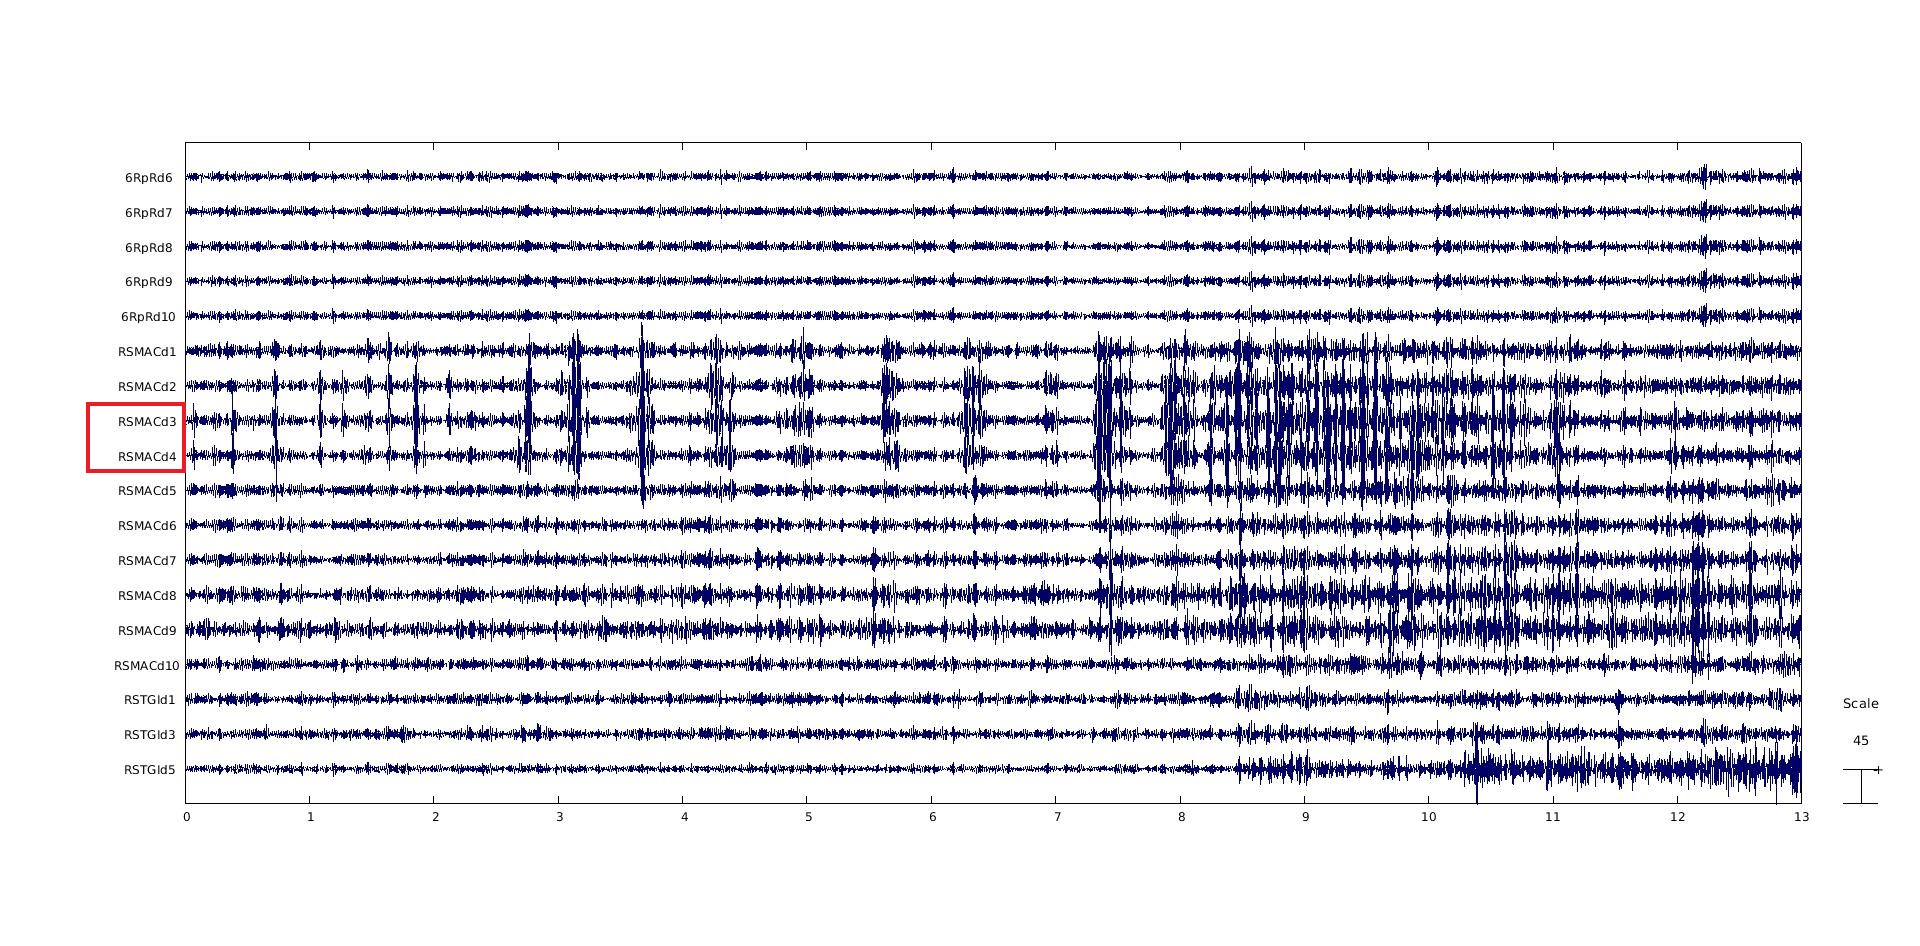
\includegraphics[height =3.5in]{Plots/Patient_C_HFO_Filtered.jpg}
	}
	\caption{13s high pass filtered iEEG time-series. High frequency activities ($> 50 Hz$ to Nyquist frequency) are visible on seizure onset electrodes RSMAcd3 and RSMAcd4 and later extended to other electrodes.}
	\label{fig:high_pass_filtered_preictal_patient_c}
\end{figure*}


\begin{figure*}
\centerline{
	\includegraphics[height =3in]{Plots/Patient_C_infraslow_100s.jpg}
	}
	\caption{100s low pass filtered iEEG time series (0.01-0.1 Hz). Infraslow activity is visible in SO electrode RSMAcd4.}
	\label{fig:infraslow_wave_patient_c}
\end{figure*}



\begin{figure}%
    \centering
    [\centering a]{{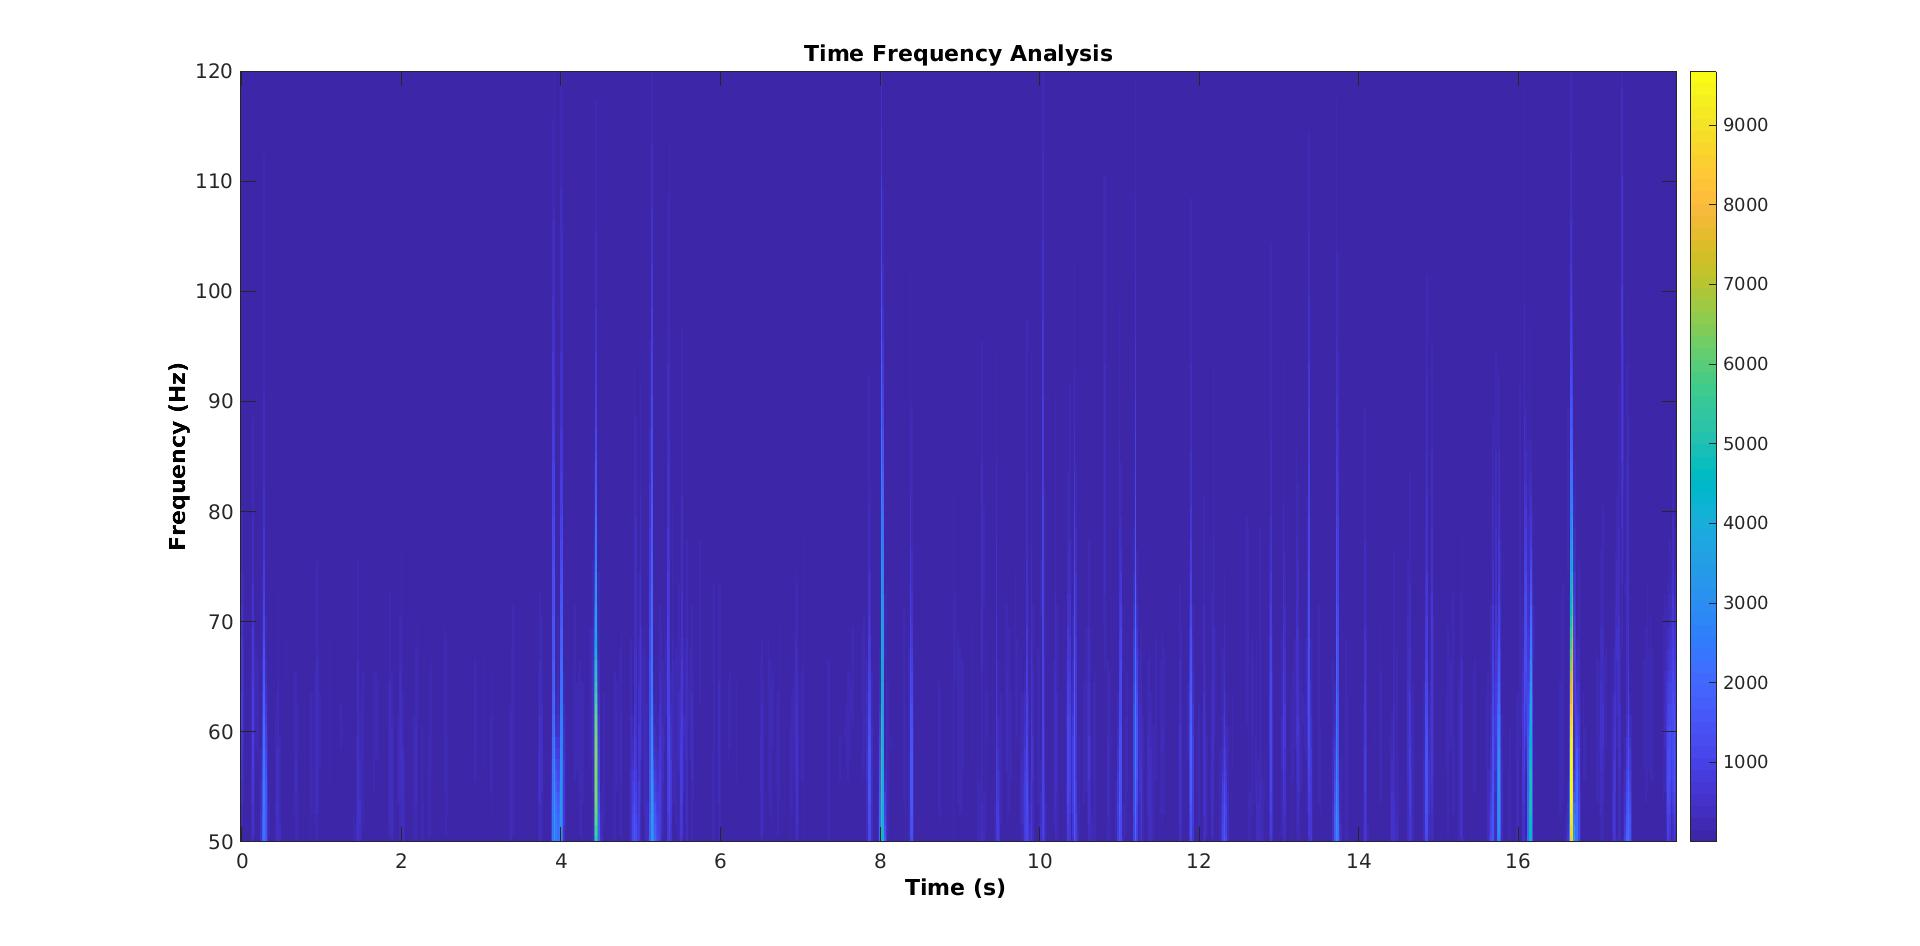
\includegraphics[width=15cm]{Plots/Time_Frequency_HFO_RSMAcd4.jpg} }}%
    \qquad
    [\centering b]{{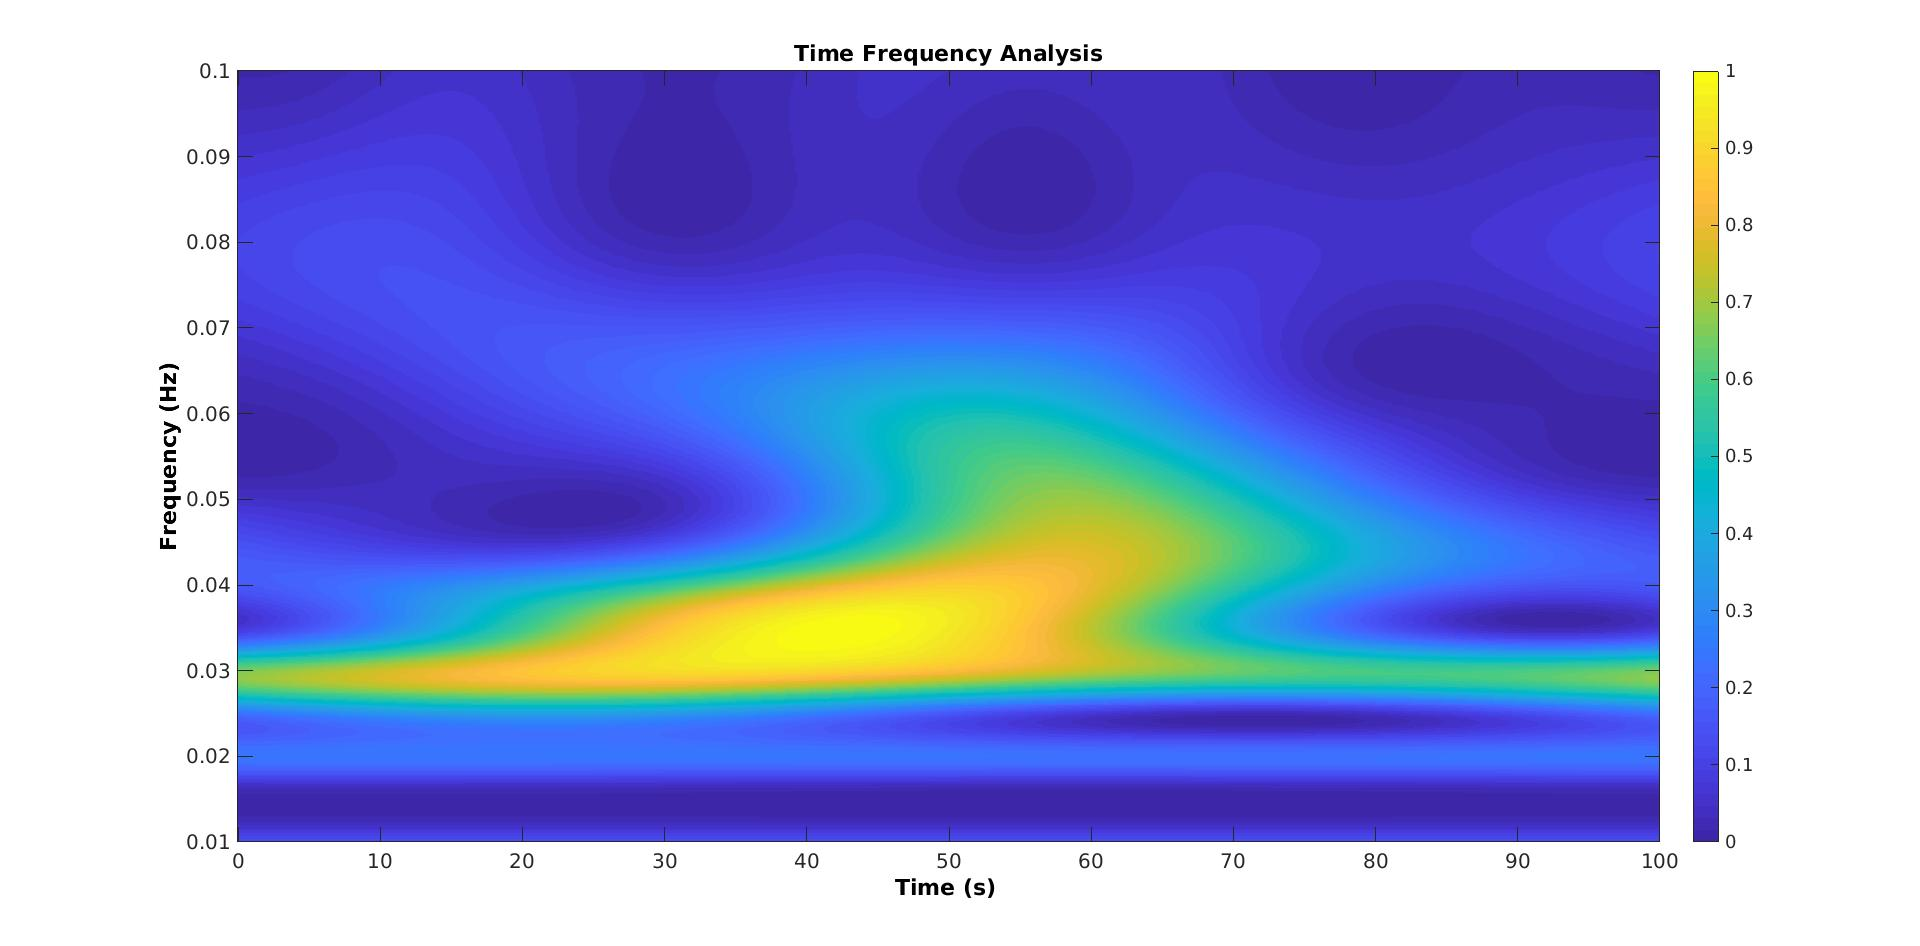
\includegraphics[width=15cm]{Plots/RSMAcd4_powerplot_infraslow_interictal.jpg} }}%
    \caption{High frequency activities as observed in representative patient on SO electrode, RSMAcd4. Scattered blobs of high frequency activity could be seen from 50 Hz-100 Hz. Time frequency analysis was done on iEEG time-series a few seconds before clinical seizure onset b) Wavelet power was computed on 100s iEEG time-series hours away from any seizure activity (inter-ictal state) for SO electrode RSMAcd4. The power was normalized between 0 and 1. Wavelet power was maximum between 10s and 70s and in the frequency range of 0.03 Hz and 0.05 Hz.}%
    \label{fig:power_plot}%
\end{figure}



\subsection{Granger causality and graph measures}
We studied characteristics of high frequency and infra-slow oscillations by computing GC spectra, source, sink and total causal flow. Neuronal information flow from the electrode to all other electrodes is called outflow or source. Similarly, neuronal information flow from all other electrodes to this electrode is termed inflow or sink activity. Total Granger causality is the sum of inflow and outflow. 

%High frequency oscillations
These measures were computed from high pass filtered iEEG time series above 50Hz to just below the Nyquist frequency with a frequency resolution of 1 Hz for HFO analysis. 
%Temporal mean was removed from the data prior to GC calculations

Figure \ref{fig:patient_c_preictal_high} shows the GC (sink and total GC) for HFOs in preictal period for a representative patient. Sink activities are visualized in the negative axis to represent incoming neuronal information flow. Red circles in the figure, denoting SO electrodes as confirmed visually by the epileptologists, were ranked in the top 5, out of 119 electrodes for causal Sink measures. Blue circles denote the contralateral SO electrode, which interestingly are also ranked among the topmost values for total GC only. We were able to localize SO electrodes for patients A, B and C (Shown in Appendix \ref{chapter:appendix-gc-results}) using these tools and methods. Sink and total GC were also clustered around SO electrodes for these patients. 

%Infraslow oscillations
Similarly, infraslow oscillations were quantified from low pass filtered iEEG time series in the frequency range 0.01 to 0.1 Hz with 1/1000 frequency resolution. Figure \ref{fig:patient_c_interictal_low} show the integrated time domain Granger causality, Sink and Total GC computed and integrated over infraslow frequency in interictal periods for the same patient. Total GC and sink activities were highly clustered around SO electrodes for this representative patient as well as two other patients (Shown in Appendix \ref{chapter:appendix-gc-results}). SO electrodes were ranked $2^{nd}$ out of 119 electrodes for both Sink and Total GC.


% \begin{figure*}
% \centerline{
% 	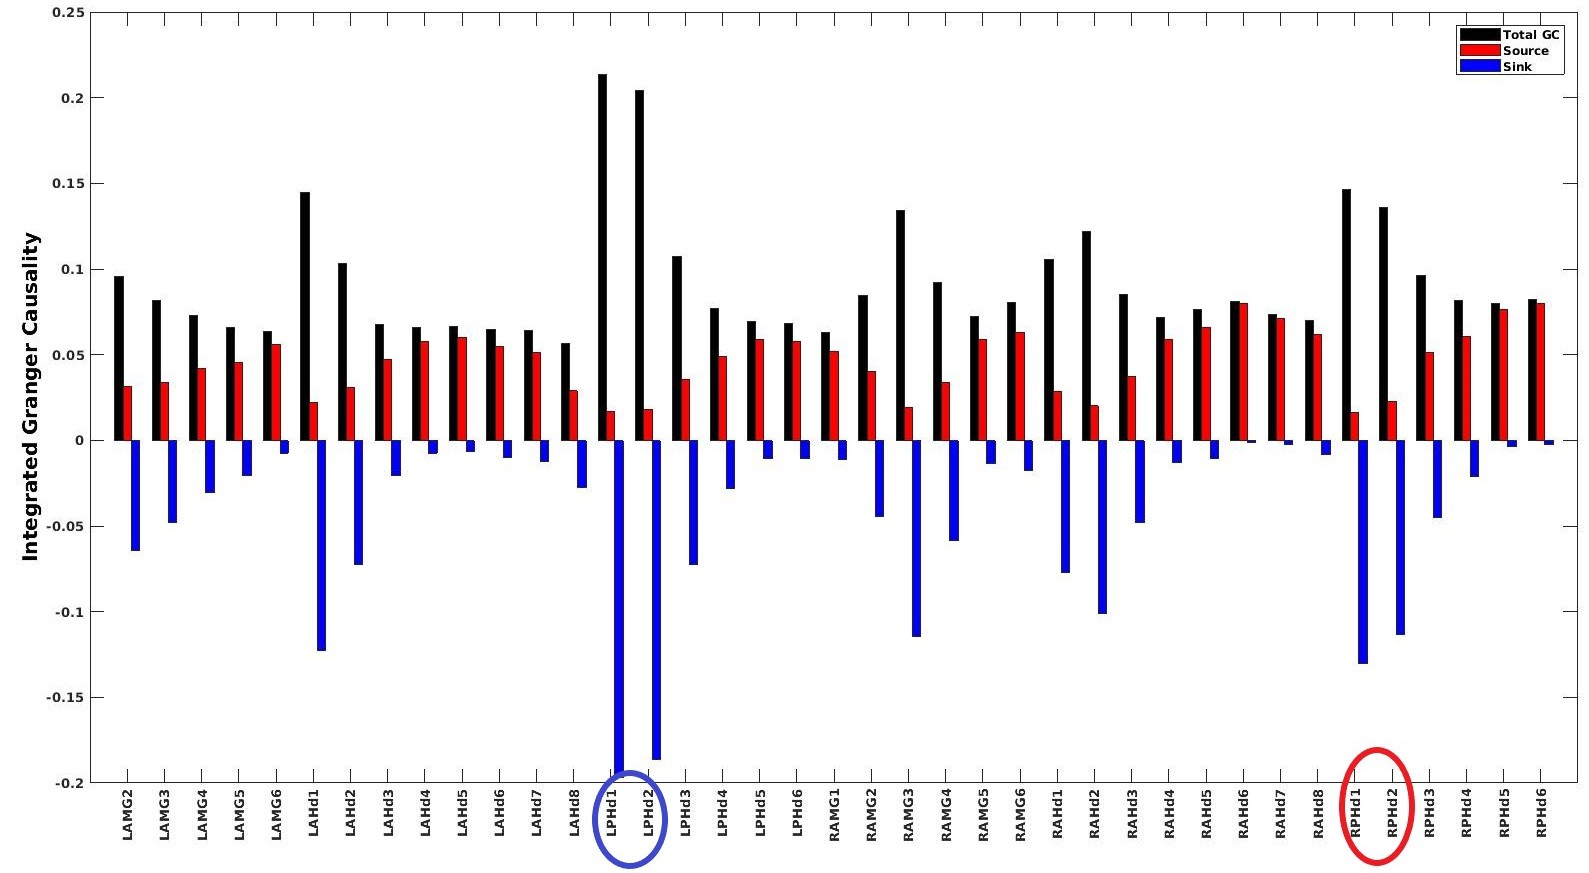
\includegraphics[height =3.5in]{Plots/Patient_A_preictal_high.jpg}
% 	}

% 	\caption{Integrated Granger Causality for preictal states for patient A. Source, sink and total were computed for 40 implanted electrodes. RpHd1 and RpHd2 are the SO electrodes on the right hemispheres. LpHd1 and LpHd2 are the contralateral electrodes. Both total GC and sink activities were maximum for contralateral electrodes and RpHd1 and RpHd2 were also ranked among the top for both total GC and sink. Source activity could not explain much about the seizure activity}

% 	\label{fig:patient_a_preictal_high}
% \end{figure*}


% \begin{figure*}
% \centerline{
% 	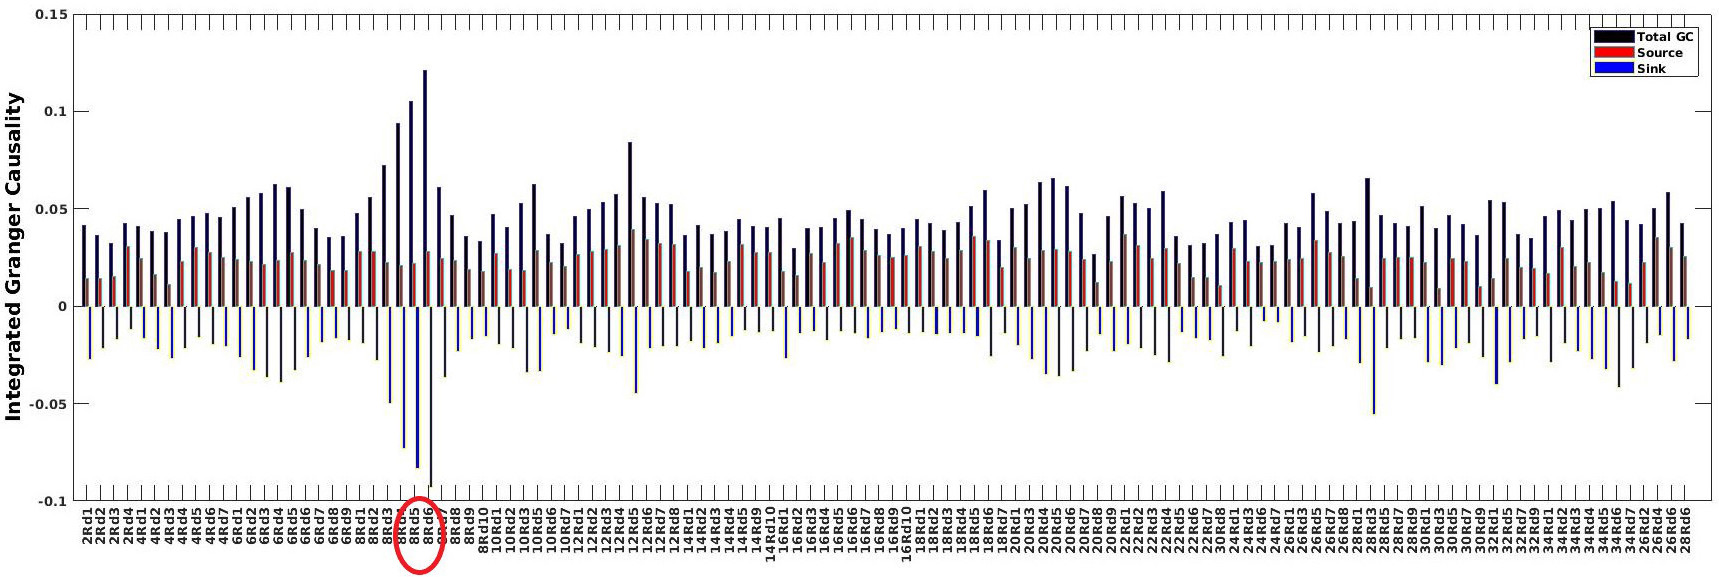
\includegraphics[height =3in]{Plots/Patient_B_preictal_high.jpg}
% 	}

% 	\caption{Integrated Granger Causality for patient B. SO electrodes 8Rd5 and 8Rd6 have very high total GC and sink measures value, suggesting that these two measures could be used for SO electrodes prediction for prospective patients}

% 	\label{fig:patient_b_preictal_high}
% \end{figure*}

\begin{sidewaysfigure*}
\centerline{
	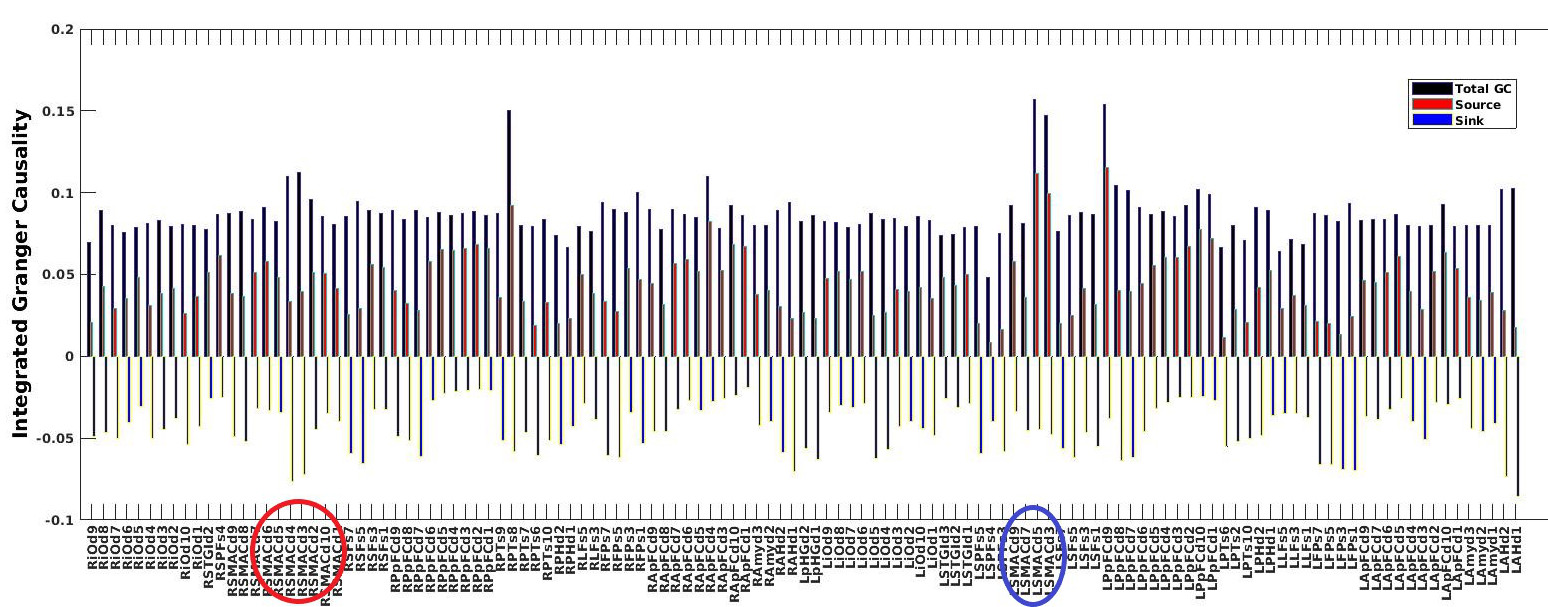
\includegraphics[height =3in]{Plots/Patient_C_preictal_high.jpg}
	}

	\caption{Integrated Granger causality of high frequency activities in preictal state for a representative patient. The SO electrodes RSMAcd are second and forth from the top for causal sink activity. The contralateral channel LSMAcd was ranked highest for Total GC.}

	\label{fig:patient_c_preictal_high}
\end{sidewaysfigure*}


\begin{sidewaysfigure*}
\centerline{
	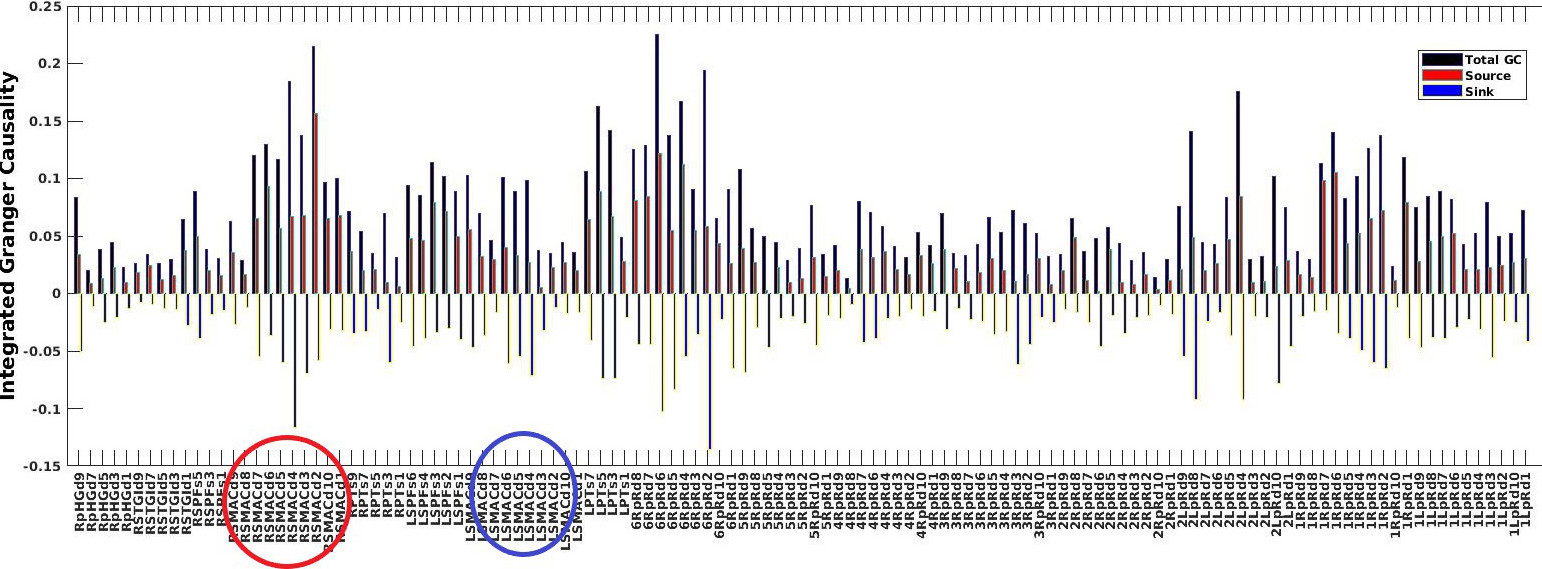
\includegraphics[height =3in]{Plots/Patient_C_interictal_low.jpg}
	}

	\caption{Integrated Granger causality of infraslow activities in the interictal state for a representative patient. The SO electrodes RSMAcd3 and RSMAcd4 are ranked at the top 2 out of 119 electrodes based upon Total GC and Sink measures. Contralateral electrodes LSMAcd3 and LSMAcd4 are much less prominent for this frequency range and state.}
	\label{fig:patient_c_interictal_low}
\end{sidewaysfigure*}

The threshold value of each integrated GC measure, for statistical significance, was computed from surrogate data methods by using data permutation calculating GC values and a gamma function fit to a distribution of maximum GC values for each permutation. This threshold was designed to reject a null hypothesis of no interdependence at a significance level of $p <10^{-6}$ as in \citep{adhikari2013localizing}.

To validate and compare the Granger causal measures, we also computed the graph theoretical measures - degree, betwenness and clustering coefficient and incloseness. Table \ref{table:summary} provides a summary view of the effectiveness of these measures along with the causal measures (Total GC and ) in localizing the seizure onset for both high and infraslow oscillations in the preictal and interictal periods. If for a particular patient, the SO electrode belongs among the top 5 for a given measure, it is considered as correct localization and counted 1, otherwise it is counted 0. Thus, the values in this table represent the number of patients for which the measure is able to localize SOZ.

As observed in the table, using the total Granger casuality, the SO electrodes were localized appropriately in all the patients for HFO in the preictal and infraslow in the interictal period. Likewise, sink and betweenness measures could predict the SO electrodes in preictal periods for high frequency only. These results suggest that either total or negative causal flow (sink), or betweenness measures could correlate seizure focus in different patients and different phases of epilepsy cycle in both high and infraslow frequency.



\begin{table}[]
\renewcommand{\arraystretch}{1.2} % Default value: 1
\setlength{\tabcolsep}{12pt} % Default value: 6pt
\centering
	\begin{tabular}{|l |c|c|c|c|}
	\hline
	  & \multicolumn{2}{c|}{\textbf{High}} & \multicolumn{2}{c|}{\textbf{Infraslow}} \\ \cline{2-5}
	\multirow{-2}{*}{\textbf{Measures}} & Preictal        & Interictal       & Preictal       & Interictal       \\ 
	\hline
	\textbf{Total GC}                   & 3               & 2                & 2              & 3                \\ \hline
	\textbf{Sink}                       & 3               & 2                & 1              & 2                \\ \hline
	\textbf{Betweenness}                & 3               & 2                & 1              & 1                \\ \hline
	\textbf{Degree}                     & 2               & 2                & 2              & 2                \\ \hline
	\textbf{Clustering coef}            & 0               & 1                & 0              & 1                \\ \hline
	\textbf{Incloseness}                & 1               & 0                & 2              & 1                \\ \hline
	\end{tabular}

	\caption{Summary listing the no. of patients for which corresponding causal and graph measures are able to localize the SO electrodes across preictal and interictal periods, in high frequency and infraslow oscillations}
	\label{table:summary}
\end{table}


\section{Discussion}
\label{sec:discussion}
In this work, we confirmed the existence of a stable iEEG network in very low to very high frequencies throughout multiple phases of focal epilepsy, from preictal to interictal, to visible ictus, using quantitative analysis methods based on spectral interdependency measures including GC spectra computation and graph measures. These network features were identified from among large sets of iEEG electrodes in selected patients who experienced sustained remission following focal invasive procedures and lacked obvious anatomic lesions. In addition to the seizure-onset patterns on iEEG, remission confirmed the accuracy of seizure localization.  Absence of anatomic lesions helps exclude the alternative possibility that focal changes in infraslow activity might be due simply to the lesion rather than to the presence of an epileptic focus.

The statistical connectivity results of integrated GC and graph measures suggested the extensive spatial-temporal neurophysiological network and its relationship to the site of focal seizure onsets both in the infra-slow frequency (0.01-0.1 Hz) and the high frequency ($> 50 Hz$ to Nyquist frequency).  Although the amplifiers in digital EEG recording equipment may lack the specific characteristics considered desirable for true DC recording, no fixed high pass filter appeared to be present, and activity below 0.1 Hz was quantified through methods of frequency analysis. 

Both sink and total GC activity were ranked among the top for all three patients for HFOs, but for infraslow activity, only total GC could localize SO electrodes, mostly in interictal periods. This could be explained on the hypothesis that during the preictal period, seizure onset zone is subject both the uncontrolled hyperactivity and increased external inhibition, which may fluctuate over time scales much briefer than this analysis., and produce maximum sink activities in these electrodes. This has been illustrated  in \citep{epstein2014application}. For interictal infraslow activity, the time duration of the measured signal is orders of magnitude is orders of magnitude slower than the feedback loops of much neuronal activity, so that infraslow measures would show only net effects. Our results suggest that total causal flow (sum of source and sink) could be higher for these nodes in interictal periods. Other groups have reported sink activity, but not that it could be either that or total \citep{narasimhan2020seizure}. The graph measures for corresponding periods could be explained on a similar hypothesis, as these were derived from the GC connectivity matrix. 

%This activity identifies the location of the epileptic seizure focus within the human brain both immediately prior to the visible seizure onset (preictal) and remotely (interictally), many hours from any visible seizure. 

The methods and results discussed in this study do not test the utility of infraslow iEEG in predicting surgical outcomes. However, they supplement the findings of larger surgical series \citep{narasimhan2020seizure, david2011imaging}, which indicate that interictal EEG networks may contribute valuable information to the epilepsy surgery assessment, thereby substantially reducing the time, risk, and cost of diagnostic pre-surgical testing. Given the relatively high voltages intrinsic to infraslow iEEG, both intracranially and at the scalp, there may be further potential for a robust and independent contribution to localization of the seizure focus. Extending the representation seizures networks to a wider range of frequencies may also extend their eventual utility for diagnosis and treatment. 